\documentclass[10pt]{article}
\usepackage[margin=1in, paperwidth=8.5in, paperheight=11in]{geometry}
\usepackage{ifpdf, amsmath, amssymb, comment, color, graphicx, stmaryrd, setspace, enumitem, fancyhdr, wrapfig, textcomp, mathptmx, siunitx, multicol}
\usepackage{hyperref}
\hypersetup{
    colorlinks=true,
    urlcolor=blue,
}

\usepackage{tikz}
\usetikzlibrary{trees}

\setlength{\headheight}{14.5pt}
\newcommand{\del}{\nabla}
\newcommand{\Q}{\mathbb{Q}}
\newcommand{\R}{\mathbb{R}}
\newcommand{\Z}{\mathbb{Z}}
\newcommand{\vu}{\mathbf{u}}
\newcommand{\vv}{\mathbf{v}}
\newcommand{\vw}{\mathbf{w}}
\newcommand{\vi}{\mathbf{i}}
\newcommand{\vj}{\mathbf{j}}
\newcommand{\vk}{\mathbf{k}}
\newcommand{\vn}{\mathbf{n}}
\newcommand{\vr}{\mathbf{r}}
\newcommand{\vs}{\mathbf{s}}
\newcommand{\va}{\mathbf{a}}
\newcommand{\vF}{\mathbf{F}}
\newcommand{\vL}{\mathbf{L}}
\newcommand{\vT}{\mathbf{T}}
\newcommand{\vN}{\mathbf{N}}
\newcommand{\vB}{\mathbf{B}}
\newcommand{\comp}{\operatorname{comp}}
\newcommand{\proj}{\operatorname{proj}}
\newcommand{\orth}{\operatorname{orth}}
\newcommand\dotp[1][.5]{\,\mathbin{\vcenter{\hbox{\scalebox{#1}{$\bullet$}}}}\,}


\newenvironment{red}{\color{red}}{\ignorespacesafterend}
\newcommand{\blue}[1]{\textcolor{blue}{#1}}
\newcommand{\green}[1]{\textcolor{green}{#1}}
\renewcommand{\section}[1]{\begin{center} \textbf{#1} \\\end{center}}
%
\hyphenpenalty=5000
\setlength{\parindent}{0in}
%\oddsidemargin=-.25in
\allowdisplaybreaks
\pagestyle{fancy}
\renewcommand{\headrulewidth}{0pt}
\lhead{MATH 203}
\rhead{Fall 2024}
%\lfoot{}
%\cfoot{}

\begin{document}
%


%\onehalfspacing
\allowdisplaybreaks
%##################################################################
\section{PS\#7 -- Chain rule - \red{Answer key} }

\begin{enumerate}[leftmargin=0pt]
    
    \item (\href{https://activecalculus.org/multi/S-10-5-Chain-Rule.html#S-10-5-Chain-Rule-7-13}{AC Multi 10.5 Exercise 13}) Suppose that $T = x^2 + y^2 - 2z$ where
    \begin{align*}
    x &= \rho\sin(\phi)\cos(\theta)\\
    y &= \rho\sin(\phi)\sin(\theta)\\
    z &= \rho\cos(\phi)
    \end{align*}
    \begin{enumerate}
        \item[a.] Construct a tree diagram representing the dependencies among the variables.
        
        \begin{red}
        \begin{center}
        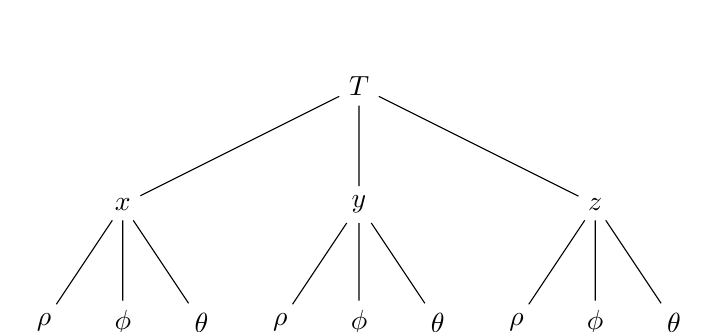
\begin{tikzpicture}[level distance=1.5cm,
          level 1/.style={sibling distance=3cm},
          level 2/.style={sibling distance=1cm}]
          \node {$T$}
            child {node {$x$}
              child {node {$\rho$}}
              child {node {$\phi$}}
              child {node {$\theta$}}
            }
            child {node {$y$}
              child {node {$\rho$}}
              child {node {$\phi$}}
              child {node {$\theta$}}
            }
            child {node {$z$}
              child {node {$\rho$}}
              child {node {$\phi$}}
              child {node {$\theta$}}
            };
        \end{tikzpicture}
        \end{center}
        (In case you're curious, I generated this tree diagram using the very good TikZ library ``trees''. I can share the LaTeX source if you're interested.)
        \end{red}
        
        
        \item[b.] Apply the chain rule to find the partial derivatives $\dfrac{\partial T}{\partial\rho}$, $\dfrac{\partial T}{\partial\phi}$, and $\dfrac{\partial T}{\partial\theta}$.
        
        \begin{red}
        We'll just read the chain rule off the tree:
        \begin{align*}
            \dfrac{\partial T}{\partial\rho} &= 
            \dfrac{\partial T}{\partial x}\cdot
            \dfrac{\partial x}{\partial\rho}
            + 
            \dfrac{\partial T}{\partial y}\cdot
            \dfrac{\partial y}{\partial\rho}
            + 
            \dfrac{\partial T}{\partial z}\cdot
            \dfrac{\partial z}{\partial\rho} \\
            &= 2x\cdot(\sin\phi\cos\theta) 
            + 2y\cdot(\sin\phi\sin\theta)
            -2\cdot(\cos\phi) \\
            &= 2(\rho\sin\phi\cos\theta)\cdot(\sin\phi\cos\theta) 
            + 2(\rho\sin\phi\sin\theta)\cdot(\sin\phi\sin\theta)
            -2\cdot(\cos\phi) \\
            &= 2\rho\sin^2\phi\cos^2\theta + 2\rho\sin^2\phi\sin^2\theta - 2\cos\phi \\
            &= 2\rho\sin^2\phi(\cos^2\theta+\sin^2\theta) - 2\cos\phi \\
            &= 2\rho\sin^2\phi-2\cos\phi
            \\
            \dfrac{\partial T}{\partial\phi} &= 
            \dfrac{\partial T}{\partial x}\cdot
            \dfrac{\partial x}{\partial\phi}
            + 
            \dfrac{\partial T}{\partial y}\cdot
            \dfrac{\partial y}{\partial\phi}
            + 
            \dfrac{\partial T}{\partial z}\cdot
            \dfrac{\partial z}{\partial\phi} \\
            &= 2x\cdot(\rho\cos\phi\cos\theta)
            + 2y\cdot(\rho\cos\phi\sin\theta)
            -2  \cdot(-\rho\sin\phi) \\
            &= 2(\rho\sin\phi\cos\theta)\cdot(\rho\cos\phi\cos\theta)
            + 2(\rho\sin\phi\sin\theta)\cdot(\rho\cos\phi\sin\theta)
            +2  \rho\sin\phi \\
            &= 2\rho^2\sin\phi\cos\phi \cdot (\cos^2\theta + \sin^2 \theta) + 2\rho\sin\phi \\
            &= 2\rho^2\sin\phi\cos\phi + 2\rho\sin\phi
            \\
            \dfrac{\partial T}{\partial\theta} &= 
            \dfrac{\partial T}{\partial x}\cdot
            \dfrac{\partial x}{\partial\theta}
            + 
            \dfrac{\partial T}{\partial y}\cdot
            \dfrac{\partial y}{\partial\theta}
            + 
            \dfrac{\partial T}{\partial z}\cdot
            \dfrac{\partial z}{\partial\theta} \\
            &= 2x\cdot(\rho\sin\phi(-\sin\theta)) 
            + 2y\cdot(\rho\sin\phi\cos\theta)
            -2 \cdot (0) \\
            &= -2(\rho\sin\phi\cos\theta)\cdot(\rho\sin\phi\sin\theta) 
            +2(\rho\sin\phi\sin\theta)\cdot(\rho\sin\phi\cos\theta) \\
            &= -2\rho^2\sin^2\phi\cos\theta\sin\theta + 2\rho^2\sin^2\phi\sin\theta\cos\theta = 0
        \end{align*}
        \end{red}
    \end{enumerate}
\end{enumerate}

\end{document}